\documentclass[a4paper, 12pt]{article}

\usepackage[T2A]{fontenc}
\usepackage[utf8]{inputenc}
\usepackage[russian]{babel}
\usepackage{graphicx}
\usepackage[normalem]{ulem}
\graphicspath{{img/}}
\DeclareGraphicsExtensions{.pdf,.png,.jpg}

\usepackage[left=3cm, right=1cm, top=2cm, bottom=2cm, bindingoffset=0cm]{geometry}

\usepackage{setspace}
\usepackage{pdflscape}
% \usepackage[nodisplayskipstretch]{setspace}

\usepackage{longtable}
\linespread{1.3}
\usepackage{indentfirst}
\setlength{\parindent}{1.25cm}
\usepackage{mathtools}

\usepackage{caption}
\DeclareCaptionLabelFormat{gostfigure}{Рисунок #2}
\captionsetup*[figure]{labelformat=gostfigure}

\usepackage{hyperref}
\usepackage{xcolor}

\usepackage{color}
\usepackage{listings} %% собственно, это и есть пакет listings
\definecolor{darkgreen}{rgb}{0,0.5,0}

\sloppy

\definecolor{linkcolor}{HTML}{000000} % цвет ссылок
\definecolor{urlcolor}{HTML}{000000} % цвет гиперссылок

\newcommand*{\undertext}[2]{%
	\begin{tabular}[t]{@{}c@{}}%
		#1\\\relax\scriptsize(#2)%
	\end{tabular}
}

\usepackage{titlesec}

\titleformat{\section}[block]
{\bfseries\large\center}{\thesection}{1em}{}
\titlespacing\section{\parindent}{3mm}{3mm}

\titleformat{\subsection}[hang]
{\bfseries\large}{\thesubsection}{1em}{}
\titlespacing\subsection{\parindent}{\parskip}{\parskip}

\titleformat{\subsubsection}[hang]
{\bfseries\large}{\thesubsubsection}{1em}{}
\titlespacing\subsubsection{\parindent}{\parskip}{\parskip}
 
\hypersetup{pdfstartview=FitH,  linkcolor=linkcolor,urlcolor=urlcolor, colorlinks=true} 
% \renewcommand{\labelenumi}{\theenumi)}

\begin{document}
\lstset{ %
language=C,                 % выбор языка для подсветки (здесь это С)
basicstyle=\footnotesize, % размер и начертание шрифта для подсветки кода
numbers=left,               % где поставить нумерацию строк (слева\справа)
numberstyle=\tiny\color{purple},           % размер шрифта для номеров строк
commentstyle = \color{darkgreen},
keywordstyle = \color{blue},
stepnumber=1,                   % размер шага между двумя номерами строк
numbersep=5pt,                % как далеко отстоят номера строк от подсвечиваемого кода
backgroundcolor=\color{white}, % цвет фона подсветки - используем \usepackage{color}
showspaces=false,            % показывать или нет пробелы специальными отступами
showstringspaces=false,      % показывать или нет пробелы в строках
showtabs=false,             % показывать или нет табуляцию в строках
frame=single,              % рисовать рамку вокруг кода
tabsize=4,                 % размер табуляции по умолчанию равен 2 пробелам
captionpos=t,              % позиция заголовка вверху [t] или внизу [b] 
breaklines=true,           % автоматически переносить строки (да\нет)
breakatwhitespace=false, % переносить строки только если есть пробел
escapeinside={\%*}{*)},   % если нужно добавить комментарии в коде
texcl=true
}
\begin{titlepage}
	\noindent \begin{minipage}{0.13\textwidth}
	
\includegraphics[width=\linewidth]{bauman_logo}
	\end{minipage}
	\noindent\begin{minipage}{0.87\textwidth}\centering
		\textbf{Министерство науки и высшего образования Российской Федерации}\\
		\textbf{Федеральное государственное бюджетное образовательное учреждение высшего образования}\\
		\textbf{~~~«Московский государственный технический университет\\имени Н.Э.~Баумана}\\
		\textbf{(национальный исследовательский университет)»}\\
		\textbf{(МГТУ им. Н.Э.~Баумана)}
	\end{minipage}
	\begin{normalsize}
	\noindent\rule{17cm}{3pt}
	\newline\newline
	\noindent ФАКУЛЬТЕТ $\underline{\text{«Информатика и системы управления»}}$ \newline\newline
	\noindent КАФЕДРА $\underline{\text{«Программное обеспечение ЭВМ и информационные технологии»}}$\newline\newline
	
	\vspace{\baselineskip}
\begin{center}
	\fontsize{22pt}{\baselineskip}\selectfont \textbf{РАСЧЕТНО-ПОЯСНИТЕЛЬНАЯ ЗАПИСКА}\\
	\fontsize{20pt}{\baselineskip}\selectfont \textit{К КУРСОВОЙ РАБОТЕ}\\
	\fontsize{20pt}{0.7\baselineskip}\selectfont \textit{НА ТЕМУ:}
\end{center}
\newcommand{\termtitle}{\textbf{Разработка базы данных для хранения}
 и аналитики результатов статистического опроса}


\begin{center}
    \fontsize{20pt}{\baselineskip}\selectfont
    \noindent <<Библиотечная система бронирования>> \hfill \\
    \fontsize{20pt} {\baselineskip} \selectfont \hfill        
\end{center}

\vspace{4cm}


\noindent Студент~~~\uline{\undertext{~~~ИУ7-23М~~~}{Группа}} \hfill 
\uline {\undertext {\mbox{\hspace*{3cm}}}{Подпись, дата}}~~~
\uline {\undertext {~~~Н. Р. Трошкин~~~}{И.О. Фамилия}}\\
Руководитель курсовой работы\hfill 
\uline{\undertext{\mbox{\hspace*{3cm}}}{Подпись, дата}}~~~
\uline{\undertext{~~А. А. Ступников~~}{И.О. Фамилия}}\\

\mbox{}
\vfill
	\begin{center}
		\vfill
		Москва~---~\the\year
		~г.
	\end{center}
	\end{normalsize}
\end{titlepage}
\newpage
\setcounter{page}{3}
\begin{large}
    \section*{РЕФЕРАТ}
\addcontentsline{toc}{section}{РЕФЕРАТ}
Расчетно-пояснительная записка 28 с., 8 рис., 1 табл., 17 ист.

Курсовая работа представляет собой разработку модели, позволяющей по тексту статьи на английском языке подобрать к ней один или несколько тегов. 
Проводится обзор и сравнение методов векторизации текста и моделей многозначной классификации для решения поставленной задачи. 
Разрабатывается программное обеспечение, реализующее методы векторизации TF-IDF и Word2Vec, а также два разных варианта ансамбля бинарных классификаторов.
Выбираются функционалы качества и на основе разработанного ПО сравниваются несколько моделей.

КЛЮЧЕВЫЕ СЛОВА

\textit{Машинное обучение, обработка текстов, многозначная классификация, векторизация, подбор тегов, Word2Vec, TF-IDF, ансамбль классификаторов.}

\newpage
\def\contentsname{СОДЕРЖАНИЕ}
\tableofcontents

\newpage
\section*{ВВЕДЕНИЕ}
\addcontentsline{toc}{section}{ВВЕДЕНИЕ}
Фитнес-индустрия в России продолжает стремительно развиваться, фитнес перестал быть просто модным хобби и стал неотъемлемой частью здорового образа жизни.
По данным исследования, подготовленного аналитической компанией FitnessData, занимающейся исследованием рынков фитнес-услуг в России и за рубежом, объем рынка фитнес-услуг в РФ за 2023 год увеличился на 18\% и составил не менее 214 млрд рублей. 
Этот рост связан как с повышением цен на данный вид услуг (на 11-12\%), так и с повышением численности занимающихся (с 6 млн человек в 2022 г. до 6.5 млн человек в 2023 г.).

В Москве насчитывается более тысячи фитнес-клубов, и потенциальным клиентам требуется много времени, чтобы подобрать клуб, который бы лучше всего подходил под их запросы. 
По этой причине есть необходимость в агрегаторе, содержащем информацию о клубах и упрощающем поиск нужного для пользователя.

Целью данной работы является разработка распределенной системы бронирования книг в библиотеках. 
Для достижения поставленной цели необходимо решить следующие задачи:

\begin{itemize}
    \item[---] сформулировать основные требования к системе;
    \item[---] описать требования к подсистемам;
    \item[---] описать архитектуру системы, а так же сценарии её функционирования;
    \item[---] выбрать и обосновать инструменты для разработки программного обеспечения;
    \item[---] реализовать программный продукт.
\end{itemize}

\newpage
\titleformat{\section}[block]
{\bfseries\large\filright}{\thesection}{1em}{}
\section{Аналитический раздел}
\subsection{Постановка задачи}
Разрабатываемая система должна предоставлять пользователям информацию о наличии книг в библиотеках, возможность найти интересующую книгу и взять ее в библиотеке.
Если у пользователя на руках есть уже $N$ книг, то он не может взять новую, пока не сдал старые. 
Если пользователь возвращает книги в хорошем состоянии и сдает их в срок, то максимальное возможное количество книг у него на руках увеличивается.

\subsection{Описание системы}
Разрабатываемое программное обеспечение должно представлять собой распределённую систему для поиска и бронирования книг в библиотеках.

Авторизованные пользователи могут просмотреть список библиотек в городе, список книг в выбранной библиотеке, информацию по всем книгам, которые были взяты в прокат данным пользователем, свой рейтинг, а также забронировать и вернуть книгу в библиотеке. 
Неавторизованные пользователи могут только зарегистрироваться или войти в систему, если учетная запись уже существует.
Для регистрации необходимо указать следующую информацию о себе: фамилия, имя, отчество, дата рождения, номер телефона, электронная почта.


\subsection{Общие требования к системе}
Требования к системе следующие:
\begin{enumerate}
	\item Разрабатываемое ПО должно поддерживать функционирование системы в режиме 24/7/365 (24 часа, 7 дней в неделю, 365 дней в году) со среднегодовым временем доступности не менее 99.9\%. Допустимое время, в течении которого система недоступна, за год должна составлять $24\cdot365\cdot0.001=8.76$ ч.
	
	\item Время восстановления системы после сбоя не должно превышать 15 минут.
	
	\item Каждый узел должен восстанавливаться после сбоя автоматически.
	
	\item Система должна поддерживать возможность <<горячего>> переконфигурирования. Необходимо предусмотреть поддержку добавления нового узла во время работы системы без рестарта.
	
	\item Обеспечить безопасность работоспособности за счёт отказоустойчивости узлов.
\end{enumerate}

\subsection{Требования к функциональным характеристикам}
\begin{enumerate}
	\item По результатам работы модуля сбора статистики среднее время отклика системы на запросы пользователя на получение информации не должна превышать 3 секунд.
	
	\item По результатам работы модуля сбора статистики медиана времени отклика системы на запросы, добавляющие или изменяющие информацию на портале не должна превышать 5 секунд.
	
	\item Медиана времени отклика системы на действия пользователя должна быть менее 0.8 секунд при условии работы на рекомендованной аппаратной конфигурации, задержках между взаимодействующими сервисами менее 0.2 секунды и одновременном числе работающих пользователей менее 100 на каждый сервер, обслуживающий внешний интерфейс.
\end{enumerate}

\subsection{Функциональные требования к системе с точки зрения пользователя}
Система должна обеспечивать реализацию следующих функций.
\begin{enumerate}
	\item Система должна обеспечивать регистрацию и авторизацию пользователей с валидацией вводимых данных как через интерфейс приложения, так и через социальные сети.
	
	\item Система должна обеспечивать аутентификацию пользователей.
	
	\item В системе должно быть обеспечено разделение всех пользователей на три роли:
	\begin{itemize}
		\item Пользователь (неавторизированный пользователь);
		
		\item Клиент (авторизированный пользователь);
		
		\item Администратор.
	\end{itemize}
	
	\item Предоставление возможностей \textbf{Пользователю, Клиенту, Администратору} представленных в таблице \ref{tbl:user-func}.
\end{enumerate}


\begin{longtable}{|p{0.5cm}|p{15.5cm}|}
    \captionsetup{singlelinecheck=false, justification=raggedleft}
	\caption{Функции пользователей}
	\label{tbl:user-func} \\
	\hline
	
	\begin{rotatebox}[origin=r]{90}
		{ \textbf{Пользователь}}
	\end{rotatebox} 
	& 
	1. регистрация в системе; \newline
	2. авторизация в системе; \\
	\hline
	
	\begin{rotatebox}[origin=r]{90}
		{ \textbf{Клиент}}
	\end{rotatebox} 
	& 
	1. получение и изменение информации текущего аккаунта; \newline
	2. просмотр списка доступных библиотек; \newline
	3. просмотр списка книг, доступных в конкретной библиотеке; \newline
	4. просмотр всех своих бронирований; \newline
	5. просмотр информации о своем рейтинге; \newline
	6. бронирование конкретной книги в конкретной библиотеке; \newline
	7. возврат забронированной данным клиентом книги в библиотеку; \\
	\hline

	\begin{rotatebox}[origin=r]{90}
	{ \textbf{Администратор}}
	\end{rotatebox} 
	& 
	1. просмотр списка всех клиентов, зарегистрированных в системе; \newline
    2. создание новых учетных записей; \newline
	3. получение отчетов о выполненных действиях от сервиса статистики; \newline
	4. просмотр и редактирование списка доступных библиотек; \newline
	5. просмотр и редактирование списка доступных книг в конкретной библиотеке; \newline
	6. бронирование книги в библиотеке на имя любого клиента; \newline
	7. возврат книги в библиотеку от имени любого клиента; \newline
	8. изменение рейтинга любого клиента; \newline
	9. просмотр списка бронирований любого клиента; \\
	\hline
	
\end{longtable}


\subsection{Входные данные}
Входные параметры системы представлены в таблице \ref{tbl:input}.

\begin{longtable}{|p{3cm}|p{13cm}|}
    \captionsetup{singlelinecheck=false, justification=raggedleft}
	\caption{Входные данные}
	\label{tbl:input} \\
	\hline
	
	\textbf{Сущность} & \textbf{Входные данные} \\
	\hline
	\endfirsthead
	
	\hline
	\textbf{Сущность} & \textbf{Входные данные} \\
	\hline
	\endhead
	
	\hline
	\multicolumn{2}{c}{\textit{Продолжение на следующей странице}}
	\endfoot
	\hline
	\endlastfoot
	
	Клиент / Администратор
	&
	1. \textit{фамилия, имя} и \textit{отчество} не более 256 символов каждое поле; \newline
	2. \textit{дата рождения} в формате дд.мм.гггг; \newline
	3. \textit{логин} не более 80 символов; \newline
	4. \textit{пароль} не менее 8 символов и не более 128, как минимум одна заглавная и одна строчная буква, только латинские буквы, без пробелов, как минимум одна цифра; \newline
	5. \textit{номер телефона}; \newline
	6. \textit{электронная почта}; \newline
	7. \textit{роль пользователя} --- клиент или администратор; \\
	\hline
	
	Рейтинг
	& 
	1. \textit{идентификатор} пользователя; \newline
	2. \textit{логин} пользователя не более 80 символов; \newline
	3. \textit{рейтинг} --- целое число от 0 до 100; \\
	\hline
	
	Библиотека
	& 
	1. \textit{идентификатор} библиотеки; \newline
	2. \textit{UUID} библиотеки; \newline
	3. \textit{название} библиотеки не более 80 символов; \newline
	4. \textit{город}, в котором находится библиотека, не более 255 символов; \newline
	5. \textit{адрес} библиотеки не более 255 символов; \\
	\hline
	
	Книга
	&
	1. \textit{идентификатор} книги; \newline
	2. \textit{UUID} книги; \newline
	3. \textit{название} книги не более 255 символов; \newline
	4. \textit{автор} книги не более 255 символов; \newline
	5. \textit{жанр} книги не более 255 символов; \newline
	6. \textit{состояние} книги, одно из трех: EXCELLENT, GOOD, BAD; \\
	\hline
	
	Связь книги и библиотеки
	&
	1. \textit{идентификатор} книги; \newline
	2. \textit{идентификатор} библиотеки; \newline
	3. \textit{количество} экземляров книги в библиотеке; \\
	\hline
	

	Бронирование
	& 
	1. \textit{идентификатор} бронирования; \newline
	2. \textit{UUID} бронирования; \newline
	3. \textit{логин} пользователя, совершившего бронирование, не более 80 символов; \newline
	4. \textit{UUID} забронированной книги; \newline
	5. \textit{UUID} библиотеки, в которой совершено бронирование; \newline
	6. \textit{статус} бронирования, одно из трех: RENTED, RETURNED, EXPIRED; \newline
	7. \textit{дата и время} совершения бронирования; \newline
	8. \textit{дата и время}, когда истекает бронирование. \\
\end{longtable}


\subsection{Выходные параметры}
Выходными параметрами системы являются web-страницы. 
В зависимости от запроса и текущей роли пользователя они содержат следующую информацию (таблица \ref{tbl:output-data})

\begin{longtable}{|p{0.5cm}|p{15.5cm}|}
	\caption{Выходные параметры}
	\label{tbl:output-data} \\
	\hline
	
	\begin{rotatebox}[origin=r]{90}
		{ \textbf{Клиент}}
	\end{rotatebox} 
	& 
	1. список доступных библиотек в городе, в списке указывается: \newline
	• \textit{название} библиотеки; \newline
	• \textit{полный адрес} библиотеки; \newline
	• \textit{город}; \\
	\cline{2-2}
	
	&
	2. список книг в выбранной библиотеке, в котором указывается: \newline
	• \textit{название} книги; \newline
    • \textit{автор} книги; \newline
    • \textit{жанр} книги; \newline
    • \textit{состояние} книги; \newline
    • \textit{количество экземляров} книги в выбранной библиотеке.
	\\
	\cline{2-2}
	
	&
	3. список взятых пользователем в прокат книг, в котором указывается: \newline
	• \textit{статус} бронирования; \newline
	• \textit{дата начала} бронирования; \newline
	• \textit{дата окончания} бронирования; \newline
	• \textit{название} книги; \newline
	• \textit{автор} книги; \newline
	• \textit{жанр} книги; \newline
	• \textit{название} библиотеки; \newline
	• \textit{адрес} библиотеки; \newline
	• \textit{город} библиотеки; \\
	\cline{2-2}
	
	&
	4. информация о рейтинге пользователя: \newline
	• \textit{рейтинг} пользователя. \\
	\hline
	
	\begin{rotatebox}[origin=r]{90}
		{ \textbf{Администратор}}
	\end{rotatebox} 
	& 
    Страницы, аналогичные страницам, доступным клиентам, а также:
	5. список клиентов, зарегистрированных в системе: \newline
	• \textit{имя} клиента; \newline
	• \textit{логин} клиента; \newline
    • \textit{дата рождения} клиента; \newline
	• \textit{почта} клиента; \newline
	• \textit{телефон} клиента. \\
    \cline{2-2}
	
	&
	6. отчет о пришедших данных из сервиса статистики. \\
	\hline
\end{longtable}

\subsection{Топология Системы}
На рисунке \ref{fig:topology} изображён один из возможных вариантов  топологии разрабатываемой распределенной Системы.
\begin{figure}[h]
	\begin{center}
		% {\includegraphics[scale = 0.6]{img/pic/topology.pdf}}
		{\includegraphics[scale = 0.5]{img/topology.pdf}}
		\caption{Топология системы}
		\label{fig:topology}
	\end{center}
\end{figure}

Система будет состоять из фронтенда и 6 подсистем:
\begin{itemize}
	\item[---] сервис-координатор;
	\item[---] сервис авторизации;
	\item[---] сервис объектов библиотек;
	\item[---] сервис бронирования;
	\item[---] сервис рейтингов;
    \item[---] сервис статистики.
\end{itemize}
%
\textbf{Фронтенд} принимает запросы от пользователей по протоколу HTTP и анализирует их. На основе проведенного анализа выполняет запросы к микросервисам бекенда, агрегирует ответы и отсылает их пользователю. 

\textbf{Сервис-координатор} -- единая точка входа и межсервисной коммуникации. 

\textbf{Сервис авторизации} отвечает за:
\begin{itemize}
	\item[---] возможность регистрации нового клиента;
	
	\item[---] аутентификацию пользователя (клиента и администратора);
	
	\item[---] авторизацию пользователя;
	
	\item[---] изменение персональных данных пользователя;
	
	\item[---] выход из сессии.
\end{itemize}

\textbf{Сервис объектов библиотек} отвечает за хранение информации обо всех библиотеках и книгах в них. 

\textbf{Сервис бронирования} реализует следующие функции:
\begin{itemize}
	\item[---] хранение и передача информации о книгах, взятых в прокат пользователем;
	
	\item[---] бронирование новой книги в библиотеке;
	
	\item[---] возврат книги в библиотеку.
\end{itemize}

\textbf{Сервис рейтингов} реализует хранение рейтингов пользователей системы.

\textbf{Сервис статистики} получает через Kafka информацию о выполненных действиях и по этим данным строит отчет для администратора.


\subsection{Требования к программной реализации}
\begin{enumerate}
	\item Система состоит из микросервисов. Каждый микросервис отвечает за свою область логики работы приложения. Сервисы должны быть запущены изолированно друг от друга.
	\item При необходимости, каждый сервис имеет своё собственное хранилище, запросы между базами запрещены.
	\item Необходимо реализовать один web-интерфейс для фронтенда в виде SPA или мобильного клиента с обязательным использованием CSS.  Интерфейс  должен  быть  доступен  через  тонкий  клиент (браузер).
	\item Взаимодействие между сервисами осуществляется посредством HTTP-запросов и/или очереди сообщений по технологии REST.
	\item Требуется выделить Gateway Service как единую точку входа и межсервисной коммуникации. В системе не должно осуществляться горизонтальных запросов.
	\item На Gateway Service для всех операций чтения реализовать паттерн Circuit Breaker. Накапливать статистику в памяти, и если система не ответила N раз, то в N + 1 раз вместо запроса сразу отдавать fallback. Через небольшой timeout выполнить запрос к реальной системе, чтобы проверить ее состояние.
	\item При недоступности подсистем должна осуществляться деградация функциональности (если подсистема некритичная) или выдача пользователю сообщения об ошибке и полный откат операции (либо постановка запроса в очередь для повторного выполнения и возврат пользователю сообщения об успехе).
	\item Все методы /api/** (кроме /api/v1/authorize и /api/v1/callback) на всех сервисах должны быть закрыты token-based авторизацией.
	\item Если авторизация некорректная (отсутствие токена, ошибка валидации JWT токена, закончилось время жизни токена (поле exp в payload)), то отдавать 401 ошибку.
	\item Развертывание приложения выполнить с использованием Managed Kubernetes Cluster и настроить Ingress Controller (для публикации сервисов наружу можно использовать только Ingress). Для деплоя использовать helm charts, они должны быть универсальными для всех сервисов и отличаться лишь набором параметров запуска. Сервисы должны быть завернуты в docker.
\end{enumerate}

\subsection{Функциональные требования к подсистемам}
Подсистемы: фронтенд, бекенд-координатор, бекенд авторизации, бекенд объектов библиотеки, бекенд бронирования, бекенд рейтингов, бекенд статистики.

\textbf{Фронтенд} -- серверное  приложение, предоставляет пользовательский интерфейс и внешний API системы, при разработке которого нужно учитывать следующее:
\begin{itemize}
	\item[---] должен принимать запросы по протоколу HTTP и формировать ответы пользователям в формате HTML;
	
	\item[---] в зависимости от типа запроса должен отправлять последовательные запросы в соответствующие микросервисы;
	
	\item[---] запросы к микросервисам необходимо осуществлять по протоколу HTTP;
	
	\item[---] данные необходимо передавать в формате JSON.
\end{itemize}

\textbf{Сервис-координатор} -- серверное приложение, через которое проходит весь поток запросов и ответов, должен соответствовать следующим требованиям разработки:
\begin{itemize}
	\item[---] принимать и возвращать данные в формате JSON по протоколу HTTP;
	\item[---] для всех операций чтения реализовать паттерн Circuit Breaker --- накапливать статистику в памяти, и если система не ответила N раз, то в N + 1 раз вместо запроса сразу отдавать fallback, а через небольшой timeout выполнить запрос к реальной системе, чтобы проверить ее состояние.
	\item[---] выполнять валидацию JWT токена с помощью JWKs;
	\item[---] реализовывать запросы, связанные с получением информации о книгах, библиотеках, бронированиях, пользователях и рейтинге пользователей, а также запросы статистики от администратора;
	\item[---] реализовывать бизнес-логику бронирования книги в библиотеке, в которую включается:
	\begin{itemize}
        \item[---] получение информации от пользователя о выбранной библиотеке, книге и дате окончания бронирования;
        \item[---] проверка количества книг у пользователя на руках (в состоянии RENTED);
        \item[---] проверка рейтинга пользователя (рейтинг определяет максимальное возможное количество книг у пользователя на руках);
        \item[---] если у пользователя меньше книг на руках, чем его рейтинг, запрос в сервис бронирований о создании нового бронирования;
        \item[---] запрос на изменение числа доступных экземпляров взятой книги в библиотеке, где произошло бронирование;
        \item[---] возврат пользователю информации об успешном или неуспешном бронировании.
    \end{itemize}

    \item[---] реализовывать бизнес-логику возврата книги в библиотеку, в которую включается:
	\begin{itemize}
        \item[---] получение информации от пользователя о бронировании, которое он собирается закрыть, состоянии книги и фактической дате возврата;
        \item[---] запрос на изменение статуса бронирования (возвращено или просрочено);
        \item[---] запрос на изменение числа доступных экземпляров возвращенной книги в библиотеке, куда произошел возврат;
        \item[---] если у книги ухудшилось состояние или возврат просрочен, запрос на уменьшение рейтинга пользователя на 10 за каждое условие;
        \item[---] в противном случае запрос на увеличение рейтинга пользователя \mbox{на 1}.
    \end{itemize}
\end{itemize}

\textbf{Сервис авторизации} должен реализовывать следующие функциональные возможности:
\begin{itemize}
	\item[---] принимать и возвращать данные в формате JSON по протоколу HTTP;
	\item[---] возможность регистрации нового клиента и обновление данных уже существующего;
	\item[---] выполнять функцию Identity Provider с использованием протокола OpenID Connect (scope: openid, profile, email);
	\item[---] для получения токена на Identity Provider должен быть реализован Authorization Flow (UI рассматривается как 3rd party application и авторизация пользователя так же выполняется через Authorization Flow).
\end{itemize}

\textbf{Сервис объектов библиотеки} реализует следующие функции:
\begin{itemize}
	\item[---] получение и отправка данных в формате JSON по протоколу HTTP;
	\item[---] получение таких данных, как:
	\begin{itemize}
		\item[---] список доступных библиотек в заданном городе;
		\item[---] список книг в конкретной библиотеке;
	\end{itemize}
	\item[---] валидация JWT токена с помощью JWKs.
\end{itemize}

\textbf{Сервис рейтингов} реализует функции:
\begin{itemize}
	\item[---] получение и отправка данных в формате JSON по протоколу HTTP;
	\item[---] предоставления информации об рейтинге по идентификатору пользователя;
	\item[---] валидация JWT токена с помощью JWKs.
\end{itemize}

\textbf{Сервис бронирования} должен реализовывать представленные такие функциональные возможности, как:
\begin{itemize}
	\item[---] получение и отправка ответов на запросы в формате JSON по протоколу HTTP;
	\item[---] валидация JWT токена с помощью JWKs;
	\item[---] предоставление информации о списке книг, взятых в прокат пользователем;
    \item[---] создание и обновление записей о бронировании в базе данных при взятии книги из библиотеки или возврате в библиотеку.
\end{itemize}

\textbf{Сервис статистики} получает через Kafka информацию о выполненных действиях и по этим данным строит отчет для администратора и валидирует его JWT-токен.

\newpage

\section{Конструкторский раздел}
\subsection{Описание датасета}
Для обучения и тестирования модели выбран датасет, содержащий 192368 статей на английском языке с платформы Medium [7]. 

Данные, содержащиеся в датасете, описаны в таблице \ref{table:dataset}.

\begin{table}[h!]
	\captionsetup{singlelinecheck = false, justification=raggedleft}
	\caption{Лучшие параметры для случая срочных и важных задач}
	\centering
	\begin{tabular}{| p{80px} | p{80px} | p{160px} |}
	\hline
    Название поля & Тип данных & Описание \\ \hline
    title & Строка & Заголовок статьи \\ \hline
    text & Строка & Текст статьи \\ \hline
    url & Строка & URL статьи \\ \hline
    authors & Список строк & Авторы статьи \\ \hline
    timestamp & Строка & Дата публикации \\ \hline
    tags & Список строк & Список тегов, связанных со статьей \\ \hline
    \end{tabular}
    \label{table:dataset}
\end{table}

\subsubsection{Подготовка данных}
В первую очередь, в датасете были убраны все поля, кроме текста статьи и тегов, так как теги требуется назначать, основываясь исключительно на тексте статьи.

Помимо этого, в изначальном датасете было более 40 тысяч уникальных тегов, так как у Medium нет стандартного набора тегов и к каждой статье может быть придуман любой тег.
При этом многие теги встречаются в очень малом числе статей и могли бы не попасть в тренировочную выборку, а если бы попали, то такого объема недостаточно, чтобы модель верно предсказывала соответствующий тег.
Более того, для каждого тега пришлось бы обучать классификатор, что заняло бы слишком много времени, особенно в случае их цепочки.
Поэтому было принято решение отфильтровать все теги, встречающиеся в статьях менее 1000 раз, оставив тем самым наиболее популярные.
Статьи, у которых не было оставшихся тегов, были удалены.
Таким образом, в датасете осталось 127316 статей с 98 различными тегами.

Также из текстов всех статей убраны так называемые <<стоп-слова>> --- слова, которые очень распространены, однако не влияют на смысл текстов (артикли, предлоги, союзы и т.~д.).

Входными данными при обучении являются только векторизованные тексты без тегов.
Выходными данными для каждого текста является массив из 98 значений <<истина>> или <<ложь>>, каждое из которых отвечает за то, присваивается некоторый тег статье или нет.
На основе поля tags датасета для обучения создана матрица тегов, в которой хранятся такие строки для каждого текста. 
\subsection{Описание алгоритмов}
Разрабатываемое программное обеспечение может работать в двух режимах:
\begin{enumerate}
    \item Режим обучения. Из файлов формата csv загружается предобработанный набор текстов на естественном языке и матрица тегов. На основе них выполняется обучение модели с заданными алгоритмами векторизации, классификации и долей тестовых данных. Обученная модель сохраняется в файл.
    \item Пользовательский режим. Из заданного файла загружается готовая модель, далее из файла или из командной строки вводится текст, и на основе модели программа выводит для него подходящие теги.
\end{enumerate}

Общая струкура ПО изображена на диаграмме в нотации IDEF0 [8] на рисунке \ref{idef}.

\begin{figure}[h!]
    \captionsetup{justification=centering}
    \center{\includegraphics[scale=0.55]{IDEF0-A0}}
    \caption{IDEF0-диаграмма разрабатываемого ПО}
    \label{idef}
\end{figure}

Алгоритм работы программы в пользовательском режиме приводится на рисунке \ref{user}.
Пользователю требуется ввести путь к файлу, в котором лежит текст, либо ввести его с командной строки (без символов перевода строки), а также указать путь к файлу, в котором сохранена модель, на вход которой нужно подать текст. 
Если пользователь не указывает путь к файлу, то используется путь по умолчанию.
Помимо этого, необходимо ввести метод векторизации $Vec$, которым требуется предобработать текст (в зависимости от того, какую модель пользователь выбрал).

\begin{figure}[h!]
    \captionsetup{justification=centering}
    \center{\includegraphics[scale=1]{user_mode}}
    \caption{Алгоритм работы программы в пользовательском режиме}
    \label{user}
\end{figure}

На рисунке \ref{train} показана схема работы программы в режиме обучения модели.
Пользователь может выбрать алгоритм $Vec$ векторизации текста, алгоритм $Class$ для обучения модели, а также долю тестовой выборки в датасете ($test\_size$).
Также можно указать имя и расположение файла, в который будет сохранена новая модель, и путь к файлу с датасетом.

\newpage

\begin{figure}[h!]
    \captionsetup{justification=centering}
    \center{\includegraphics[scale=1]{train_mode}}
    \caption{Алгоритм работы программы в режиме обучения}
    \label{train}
\end{figure}

\newpage

\section{Технологический раздел}
\subsection{Выбор языка и среды программирования}
В качестве языка программирования был выбран язык Python [9]. 
Язык пользуется популярностью у исследователей и разработчиков моделей машинного обучения благодаря своей простоте и лаконичности, что позволяет быстро разрабатывать сложные алгоритмы. 
Это привело к появлению множества библиотек и фреймворков, значительно упрощающих разработку программного обеспечения.

В качестве среды разработки была выбрана Visual Studio Code [10]. 
Она бесплатная, кроссплатформенная, также предоставляет возможность установки дополнений, например, подсветку синтаксиса и статический анализатор кода.

В программе были использованы следующие библиотеки:
\begin{itemize}
    \item[---] scikit-learn;
    \item[---] gensim;
    \item[---] pandas;
    \item[---] matplotlib;
    \item[---] numpy;
    \item[---] skops.
\end{itemize}
Библиотека scikit-learn [11] используется для обучения модели, так как в ней присутствуют встроенные алгоритмы для многозначной классификации, а также встроенные метрики для оценки качества полученной модели.

Библиотека gensim [12] необходима для реализации векторизации методом Word2Vec. 
Помимо инструментов для данного типа векторизации, библиотека предоставляет доступ к предобученным нейронным сетям, которые можно использовать в Word2Vec.

Библиотека pandas [13] предназначена для работы с данными. 
Она предоставляет высокоуровневые структуры данных, которые облегчают обработку, манипуляцию и анализ данных, а также включает в себя широкое множество функций для работы с ними.

Matplotlib [14] предоставляет инструменты для остроения графиков, диаграмм и других видов визуализации данных.

Skops [15] --- это библиотека, предназначенная для работы с моделями машинного обучения, созданными с использованием scikit-learn. 
Она используется для сохранения и загрузки моделей.

Библиотека numpy [16] создана для работы с массивами и матрицами, а также для выполнения математических и логических операций над ними. 
Она используется, так как поддерживается многими другими библиотеками, в том числе описанными выше.

\subsection{Код программы}

\subsubsection{Обработка текста}
В листингах 1-2 приводится код модуля, отвечающего за векторизацию текста.
Реализованы два метода векторизации --- TF-IDF и Word2Vec.
\captionsetup{singlelinecheck=false, justification=raggedleft}
\begin{lstlisting}[caption={Модуль обработки текста}]
import nltk
import re
import numpy as np
import pandas as pd

from sklearn.feature_extraction.text import TfidfVectorizer
from sklearn.preprocessing import normalize
from nltk.corpus import stopwords
from gensim.models import Word2Vec, KeyedVectors
from gensim import downloader
import skops.io as sio

stopWords = stopwords.words("english")

def delete_stop_words(text):
    return [word for word in text if word not in stopWords]

def format_data(text):
    fmtTextStr = re.sub(r'[^\w\s]', ' ', text.lower(), flags=re.UNICODE)
    tokenTextArr = nltk.word_tokenize(fmtTextStr)
    cleanTextArr = delete_stop_words(tokenTextArr)
    return " ".join(cleanTextArr)
\end{lstlisting}
\begin{lstlisting}[caption={Модуль обработки текста}]
def vectorize_tf_idf(data):
    vocabulary = None
    try:
        vocabulary = sio.load("model/vocab.skops")
    except:
        pass
    vectorizer = TfidfVectorizer(sublinear_tf=True, min_df=0.01, max_df=0.95, stop_words=stopWords, vocabulary=vocabulary)
    x = vectorizer.fit_transform(data['text'])
    sio.dump(vectorizer.vocabulary_, "model/vocab.skops")
    return x

def _preprocess(s):
    return [i for i in s.split()]

def _get_vector(s, model):
    try:
        return np.sum(np.array([model[i] for i in _preprocess(s) if i in model]), axis=0)
    except:
        return 0

def vectorize_word2vec(data):
    w2v_model = downloader.load('word2vec-google-news-300')
    x = [_get_vector(text, w2v_model) for text in data["text"]]
    return normalize(x)

def vectorize(data, mode):
    if isinstance(data, str):
        data = pd.DataFrame({"text": [data]})
    
    data["text"] = data.text.apply(lambda text: format_data(text))

    if mode == "tf-idf":
        return vectorize_tf_idf(data)

    return vectorize_word2vec(data)    
\end{lstlisting}

\subsubsection{Работа с моделями}
В листингах 3-6 приводятся фрагменты кода модуля, отвечающего за модели.
Помимо кода ниже, в модуле реализованы экспорт и импорт моделей из файлов.
\newpage
\begin{lstlisting}[caption={Обучение независимых классификаторов}]
import skops.io as sio
import numpy as np
import pandas as pd

from sklearn.multioutput import MultiOutputClassifier, ClassifierChain
from sklearn.linear_model import LogisticRegression
from sklearn.metrics import jaccard_score, precision_score, recall_score, accuracy_score
from sklearn.model_selection import train_test_split

PRED_OK = 0.5

def import_model(filename):
    unknown_types = sio.get_untrusted_types(file=filename)
    return sio.load(filename, trusted=unknown_types)

def export_model(model, filename):
    obj = sio.dump(model, filename)

def train_moc(data, labels, test_size):
    X_train, X_test, Y_train, Y_test = train_test_split(data, labels, test_size=test_size)
    clf = MultiOutputClassifier(LogisticRegression())
    model = clf.fit(X_train, Y_train)

    predicted_y = model.predict(X_test)
    Y_test_arr = np.array(Y_test).reshape(1, -1)[0]
    predicted_y_arr = predicted_y.reshape(1, -1)[0]

    return {
        "model": model,
        "precision": precision_score(Y_test_arr, predicted_y_arr),
        "recall": recall_score(Y_test_arr, predicted_y_arr),
        "accuracy": accuracy_score(Y_test_arr, predicted_y_arr),
        "jaccard": jaccard_score(Y_test_arr, predicted_y_arr)
    }

def train(data, labels, test_size, chains_amt=0):
    if chains_amt == 0:
        return train_moc(data, labels, test_size)

    return train_chain(data, labels, test_size, chains_amt)
\end{lstlisting}
\newpage
\begin{lstlisting}[caption={Обучение цепочки классификаторов}]
    def train_chain(data, labels, test_size, chains_amt):
    X_train, X_test, Y_train, Y_test = train_test_split(data, labels, test_size=test_size)
    chains = [ClassifierChain(LogisticRegression(), order="random", random_state=i) for i in range(chains_amt)]
    for chain in chains:
        chain.fit(X_train, Y_train)

    Y_pred_chains = np.array([chain.predict_proba(X_test) for chain in chains])
    Y_pred_ensemble = Y_pred_chains.mean(axis=0).reshape(1, -1)[0]
    Y_test_arr = np.array(Y_test).reshape(1, -1)[0]

    ensemble_jaccard_score = jaccard_score(
        Y_test_arr, Y_pred_ensemble >= PRED_OK
    )

    ensemble_precision_score = precision_score(
        Y_test_arr, Y_pred_ensemble >= PRED_OK
    )

    ensemble_recall_score = recall_score(
        Y_test_arr, Y_pred_ensemble >= PRED_OK
    )

    ensemble_accuracy_score = accuracy_score(
        Y_test_arr, Y_pred_ensemble >= PRED_OK
    )

    return {
        "model": chains,
        "precision": ensemble_precision_score,
        "recall": ensemble_recall_score,
        "accuracy": ensemble_accuracy_score,
        "jaccard": ensemble_jaccard_score
    }
    
\end{lstlisting}
    
\begin{lstlisting}[caption={Применение моделей}]
def to_tags_list(labels):
    tags = []
    i = 0
    for key in KEYS:
        if labels[0][i]:
            tags.append(key)
        i += 1
    return tags
\end{lstlisting}
    
\begin{lstlisting}[caption={Применение моделей}]
def predict_tags(text, model):
    if isinstance(model, list):
        Y_pred_chains = np.array([chain.predict_proba(text) for chain in model])
        return to_tags_list(Y_pred_chains.mean(axis=0).reshape(1, -1) >= PRED_OK)
    
    return to_tags_list(model.predict(text))
\end{lstlisting}

Помимо описанных выше функций в программе реализовано меню, посредством которого пользователь осуществляет ввод данных, а также управляющий модуль, который на основе введенных данных вызывает соответствующие функции.

\newpage

\section{Исследовательский раздел}
\subsection{Исследование моделей}
Так как результатом многозначной классификации является последовательность логических выражений <<истина>> и <<ложь>>, то для оценки ее точности можно использовать те же параметры, основанные на матрице ошибок, что и в классической бинарной классификации.

К этим показателям относятся [17]:
\begin{itemize}
    \item[---] точность (precision) --- показывает, сколько объектов, предсказанных положительными, действительно таковыми являются ($TP / (TP + FP)$);
    \item[---] полнота (recall) --- показывает, сколько объектов, являющихся положительными, были правильно обнаружены моделью ($TP / (TP + FN)$);
    \item[---] общая точность (accuracy) --- показывает, как часто модель предсказывает любой класс верно (доля правильных ответов, $(TP + TN) / (TP + TN + FN + FP)$);
    \item[---] f1-мера (F1-score) --- гармоническое среднее точности $p$ и полноты $r$ ($2pr/(p + r)$).
\end{itemize}

В данной задаче выходной массив можно назвать разреженным, так как в исходном датасете из 98 тегов одной статье соответствует не более 5 тегов. 
По этой причине, за счет того что подавляющее число значений в выходном векторе являются значениями <<ложь>>, значение accuracy, вероятнее всего, будет высоким, но при этом недостаточно хорошо отражающим качество модели.

На рисунке \ref{accuracy} продемонстрирован график зависимости общей точности классификации от объема обучающей выборки для разных моделей.
На нем можно видеть, что эта метрика везде приблизительно составляет 98\%.

Ниже будут рассмотрены другие показатели, которые являются более репрезентативными для данной задачи.
\newpage

\begin{figure}[h!]
    \captionsetup{justification=centering}
    \center{\includegraphics[scale=0.9]{accuracy}}
    \caption{Значение метрики accuracy для разных моделей}
    \label{accuracy}
\end{figure}

Показатель recall при многозначной классификации подходит в задачах, где очень важно обнаружить все релевантные метки и пропуск любой метки может привести к значительным негативным последствиям.
В случае определения тегов для текста вполне допустимо пропустить одну или несколько меток, сходных по значению, присвоив только некоторые. 

С другой стороны, показатель precision позволяет понимать, как часто модель ошибается, присваивая теги, которые на самом деле отсутствуют.
С точки зрения определения тегов этот показатель более информативен, так как важно присваивать метки, соответствующие материалам текста. 

Так как ранее было выяснено, что для цепочки классификаторов требуется строить несколько моделей и усреднять их для получения лучшего качества, сперва необходимо исследовать влияние числа этих моделей на результат с целью подбора оптимального.
На рисунке \ref{chains} приводится график зависимости точности результатов, предсказанных моделью, от числа цепочек в этой модели.
\newpage
\begin{figure}[h!]
    \captionsetup{justification=centering}
    \center{\includegraphics[scale=0.7]{chains}}
    \caption{Зависимость метрики precision от количества классификаторов в цепочке}
    \label{chains}
\end{figure}

Из графика следует, что примерно при 5-10 цепочках значение точности выравнивается и дальнейшее увеличение их числа уже не приводит к повышению качества модели.
Поэтому далее при сравнении моделей будет указываться результат для модели с 10 цепочками.

На рисунке \ref{precision} продемонстрирован график зависимости точности классификации от объема обучающей выборки для разных моделей.

\begin{figure}[h!]
    \captionsetup{justification=centering}
    \center{\includegraphics[scale=0.82]{precision}}
    \caption{Значение метрики precision для разных моделей}
    \label{precision}
\end{figure}

На графике можно видеть, что при выборе метода векторизации TF-IDF исследуемая метрика получается примерно на 5 процентных пунктов (или на 7.5\%) выше, чем при векторизации методом Word2Vec, и составляет примерно 70-73\%.
Также можно отметить, что наивысшая точность получается при небольшой тестовой выборке, примерно 5-10\% от общего объема датасета.
Далее происходит переобучение и точность снижается.
В то же время разница между использованием независимых классификаторов и их цепочки несущественна.

Также было вычислено значение метрики, аналогичной recall и обозначающей долю данных тестовой выборки, для которых модель верно предсказала хотя бы один тег.
Среднее гармоническое этой метрики и precision (аналог f1-меры) приводится на рисунке \ref{f1}.
При этом сохраняется тенденция метода векторизации TF-IDF к более высоким показателям качества в данной задаче, чем у Word2Vec.

\begin{figure}[h!]
    \captionsetup{justification=centering}
    \center{\includegraphics[scale=0.82]{ones}}
    \caption{Значение аналога метрики f1 для разных моделей}
    \label{f1}
\end{figure}

Таким образом, наилучшей из исследованных моделей является модель на основе векторизации TF-IDF, построенная на обучении независимых классификаторов, так как он обеспечивает тот же уровень качества, что и цепочка классификаторов, но работает быстрее за счет возможности параллелизации и отсутствия дополнительных входных параметров.

Объем тренировочной выборки можно варьировать в зависимости от целей: если не так важно определить все теги для текста, но определять их точнее, то объем тренировочной выборки может составлять около 10\% от всего датасета.
Если же важно получить более широкое множество релевантных тегов, то для повышения значения recall можно увеличить долю тренировочной выборки вплоть до 90\%.

\subsection{Демонстрация работы программы}
На рисунке \ref{tags} изображен пример вывода программы при вводе текста, взятого не из датасета и не с источника Medium.
В тексте рассказывается об особенностях экотуризма, его преимуществах и отличиях от массового туризма. 
Как можно видеть, модель распознала теги <<Окружающая среда>>, <<Изменение климата>> и <<Путешествия>>, что соответствует тематике текста.
\begin{figure}[h!]
    \captionsetup{justification=centering}
    \center{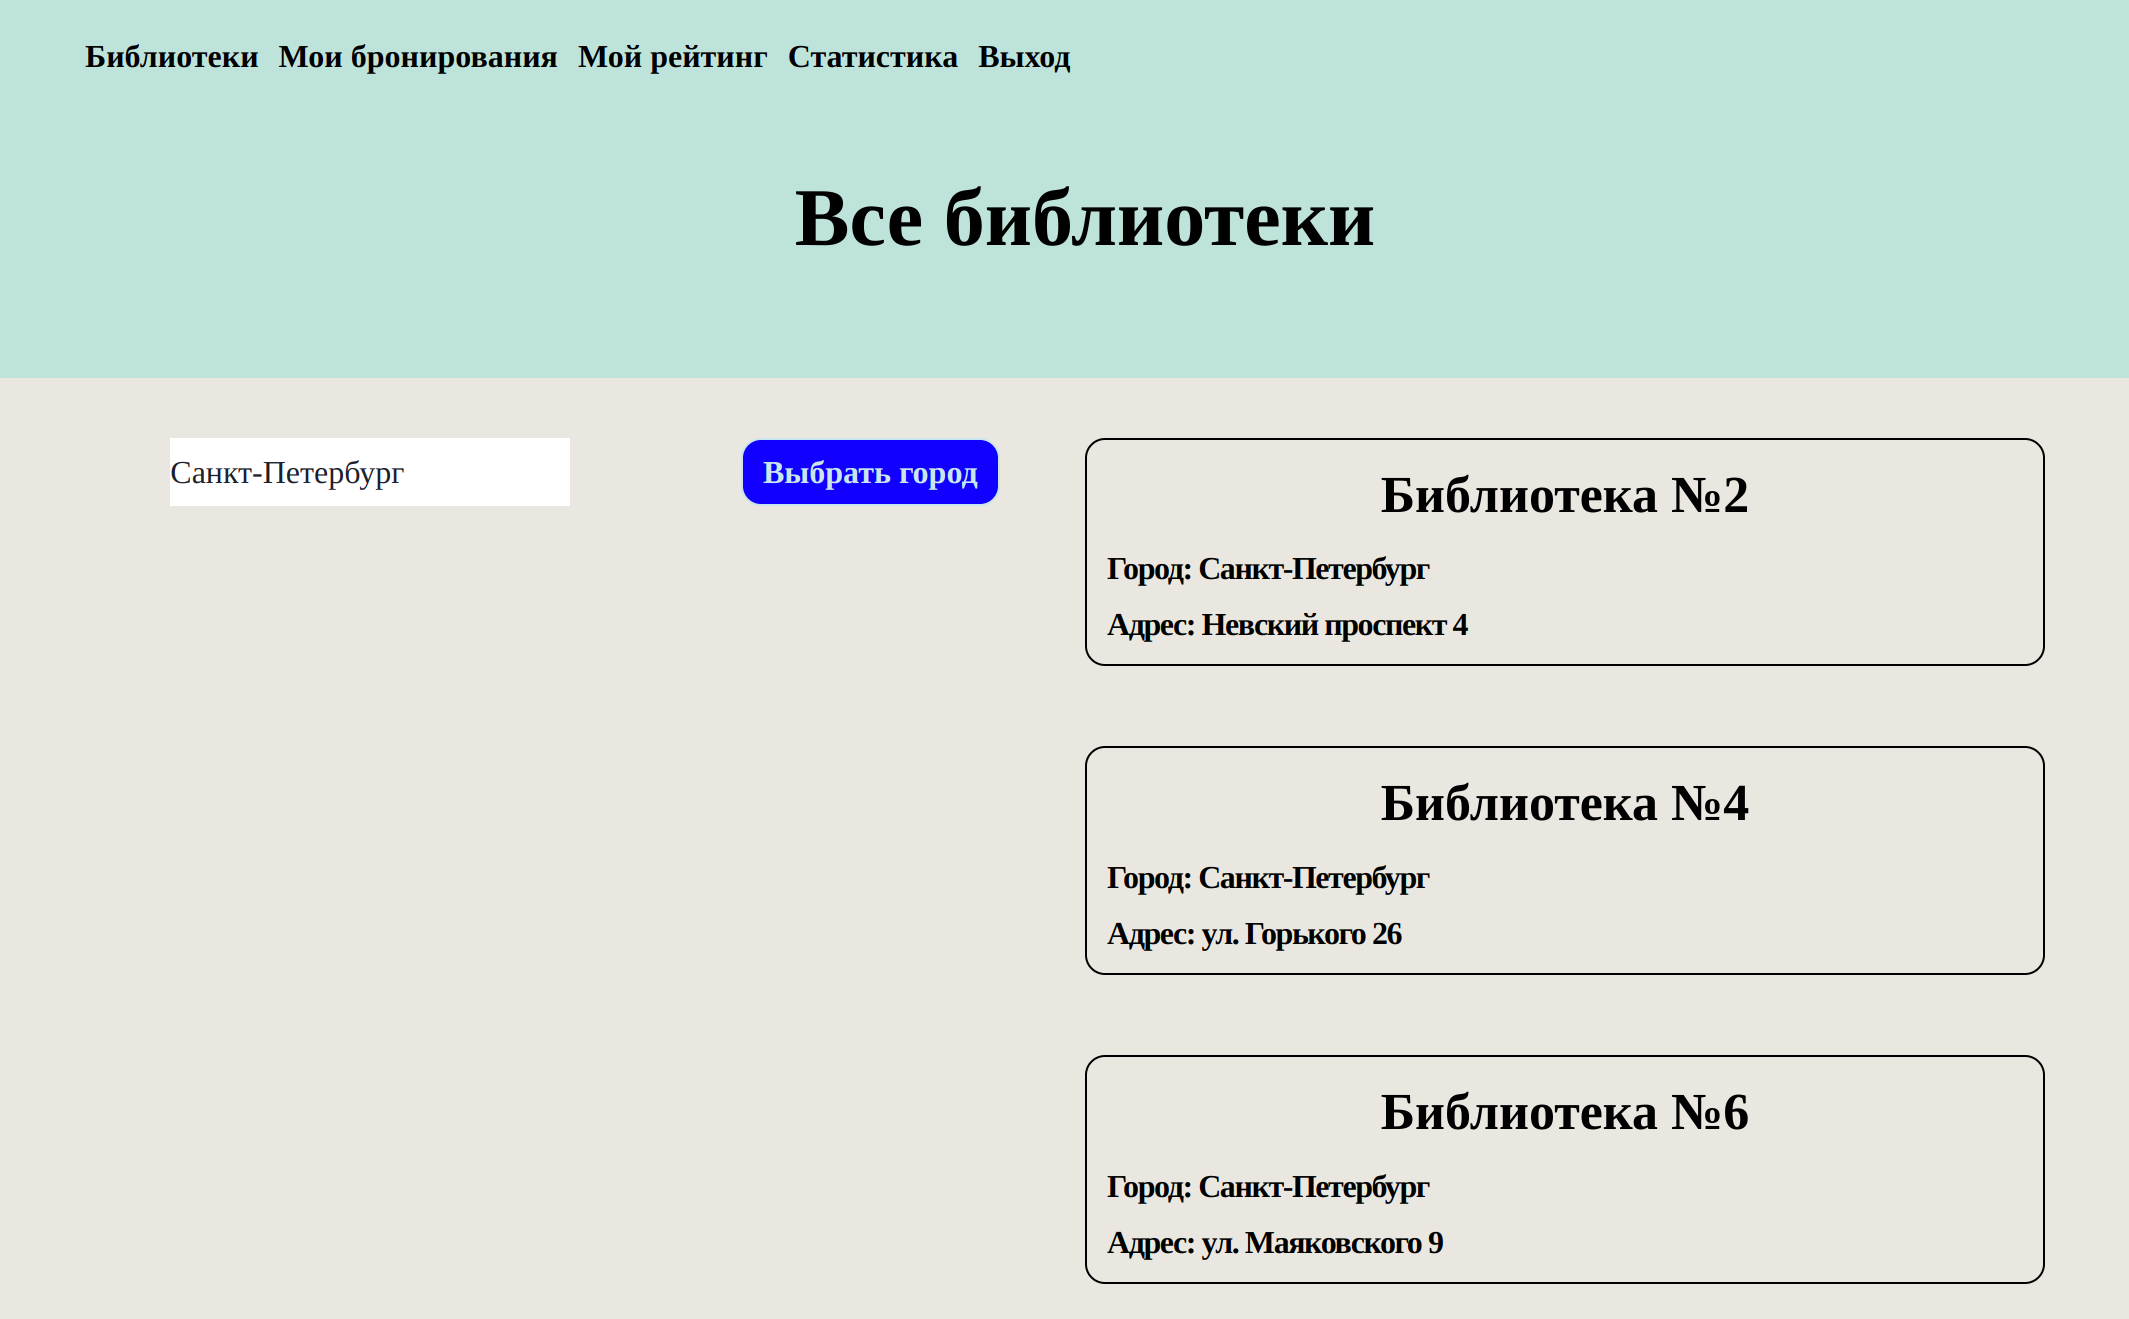
\includegraphics[scale=0.35]{interface}}
    \caption{Демонстрация работы программы}
    \label{tags}
\end{figure}

\newpage
\titleformat{\section}[block]
{\bfseries\large\center}{\thesection}{1em}{}
\section*{ЗАКЛЮЧЕНИЕ}
\addcontentsline{toc}{section}{ЗАКЛЮЧЕНИЕ}
В результате выполнения курсовой работы: 
\begin{itemize}
    \item[---] проанализированы и выбраны методы векторизации и многозначной классификации, необходимые для решения поставленной задачи;
    \item[---] описан набор данных, на которых проводилось обучение модели;
    \item[---] разработано программное обеспечение, реализующее обучение модели, а также определение тегов к произвольному тексту на основе предобученной модели;
    \item[---] выбраны метрики качества и сравнены различные реализации модели по этим метрикам.
\end{itemize}

В результате сравнения был выбран метод векторизации TF-IDF в сочетании с обучением независимых бинарных классификаторов.

Таким образом, была разработана и протестирована модель для подбора тегов к англоязычным текстам.
\newpage
\section*{СПИСОК ИСПОЛЬЗОВАННЫХ ИСТОЧНИКОВ}
\addcontentsline{toc}{section}{СПИСОК ИСПОЛЬЗОВАННЫХ ИСТОЧНИКОВ}
\begin{enumerate}
    \item Абрамов, Е. Г. Подбор ключевых слов для научной статьи / Е. Г. Абрамов // Научная периодика: проблемы и решения. --- 2011. --- № 2(2). --- С. 35-40.
    \item Кравченко, Ю. А. Векторизация текста с использованием методов интеллектуального анализа данных / Ю. А. Кравченко, А. М. Мансур, Ж. Х. Мохаммад // Известия ЮФУ. Технические науки. --- 2021. --- № 2(219). --- С. 154-167.
    \item Le Q., Mikolov T. Distributed Representations of Sentences and Documents // Proceedings of the 31st International Conference on Machine Learning. Т. 32 / под ред. E. P. Xing, T. Jebara. --- Beijing, China : PMLR, 22–24 Jun.2014. --- С. 1188—1196.
    \item Mikolov T. Efficient Estimation of Word Representations in Vector Space / T. Mikolov [и др.]. --- 2013.
    \item Jesse Read, Bernhard Pfahringer, Geoff Holmes. Classifier Chains for Multi-label Classification. --- 2009.
    \item Multiclass and multioutput algorithms --- scikit-learn 1.5.0 documentation [Электронный ресурс]. Режим доступа: \url{https://scikit-learn.org/stable/modules/multiclass.html} (дата обращения: 26.05.2024).
    \item 190k+ Medium Articles | Kaggle [Электронный ресурс]. Режим доступа: \url{https://www.kaggle.com/datasets/fabiochiusano/medium-articles} (дата обращения: 26.05.2024).
    \item РД IDEF0-2000. Методология функционального моделирования IDEF0: руководящий документ. // М.: Госстандарт России. --- 2000. --- 75 с.
    \item Our Documentation | Python.org [Электронный ресурс]. Режим доступа: \url{https://www.python.org/doc/} (дата обращения: 06.06.2024).
    \item Visual Studio Code --- Code Editing. Redefined [Электронный ресурс]. Режим доступа: \url{https://code.visualstudio.com/} (дата обращения: 06.06.2024).
    \item scikit-learn: machine learning in Python --- scikit-learn 1.5.0 documentation [Электронный ресурс]. Режим доступа: \url{https://scikit-learn.org/stable/index.html} (дата обращения: 08.06.2024).
    \item Gensim: Topic modelling for humans [Электронный ресурс]. Режим доступа: \url{https://radimrehurek.com/gensim/} (дата обращения: 08.06.2024).
    \item pandas --- Python Data Analysis Library [Электронный ресурс]. Режим доступа: \url{https://pandas.pydata.org/} (дата обращения: 08.06.2024).
    \item Matplotlib --- Visualization with Python [Электронный ресурс]. Режим доступа: \url{https://matplotlib.org/} (дата обращения: 08.06.2024).
    \item Welcome to skops's documentation! --- skops 0.9 documentation [Электронный ресурс]. Режим доступа: \url{https://skops.readthedocs.io/en/stable/} (дата обращения: 08.06.2024).
    \item NumPy [Электронный ресурс]. Режим доступа: \url{https://numpy.org/}(дата обращения --- 08.06.2024).
    \item Metrics for Multilabel Classification | Mustafa Murat ARAT [Электронный ресурс]. Режим доступа: \url{https://mmuratarat.github.io/2020-01-25/multilabel_classification_metrics} (дата обращения: 06.06.2024).
\end{enumerate}

\end{large}
\end{document}